% !TeX root = ../../../thesis.tex


\section{\acs{UEFI}/\acs{PI}}
% what is it
\textcquote{uefi-spec-overview}{The \ac{UEFI} specifications define a new model for the interface between personal-computer \ac{OS} and \ac{PF}. \textelp{} Together, these provide a standard environment for booting an \ac{OS} and running pre-boot applications}.

UEFI is pure interface spec
\cite{beyond-bios}
% why does it exist
It was designed to replace the legacy \acl{BF} \ac{BIOS}, while also often offering a backwards compatible mode with the \acf{CSM}.
% what it defines
The specification is a pure interface specification thus merely states what interfaces and structures a \ac{PF} has to offer and what an \ac{OS} may use.
% what it doesn't define
how it is implemented by PF
what is used by OS
% what does it consist of
boot- and runttime service functions for the bootloader and os to call
datatables containing platform-related information
% what are its concrete goals
- complete solution describing all features and capabilities
- abstract interfaces to support a range of processors without the need for knowledge about underlying hardware for the bootloader
- sharable persistent storage for platform support code
security

\subsection{Boot Sequence}

% https://edk2-docs.gitbook.io/edk-ii-build-specification/2_design_discussion/23_boot_sequence

focus will be on dxe and transient system load

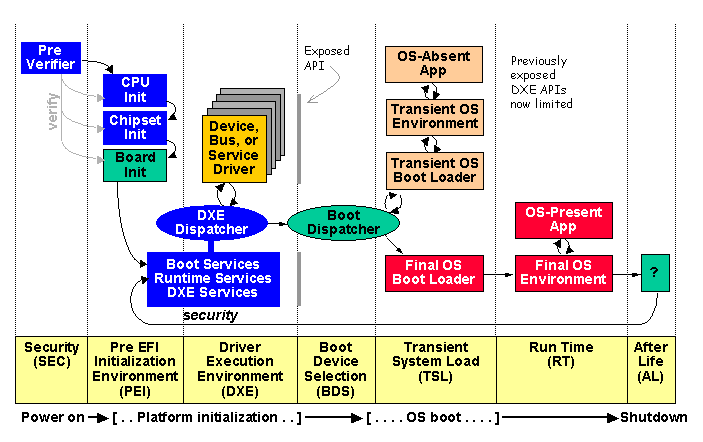
\includegraphics[width=\textwidth]{boot_sequence}


\begin{enumerate}
    \item{\acf{SEC}}

    % The SEC phase is the first phase in the UEFI boot process. It is specified in \cite[Vol 1, Section 13 ]{pi-spec}. Under its responsibilities fall setting up temporary memory used for the stack and the establishment of the system's root of trust which is a foundation for all secure operations. Inductive security designs rely on this root of trust to build a chain of trust by having a module verify the integrity of its subsequent module.
    ref to PSP

    inductive security design
    integrity of next module checked by the previous module

    handles all platform restart events
    applying power to system from unpowered state
    restarting from active state
    receiving exception conditions

    creates temporary memory store
    possibly CPU \ac{CAR}
    cache behaves as linear store of memory
    no evictions mode
    every memory access is a hit
    eviction not supported as main memory is not set up yet and would lead to platform failure


    final step
    Pass handoff information to the \ac{PEI} Foundation
    % what is the PEI foundation
    \begin{itemize}
        \item state of platform
        \item location and size of the \ac{BFV}
        \item location and size of the temporary RAM
        \item location and size of the stack
        \item optionally one or more \acp{HOB} via the \ac{SEC} \ac{HOB} Data \ac{PPI}
    \end{itemize}


    Part of this process is a so called \ac{HOB} with a function pointer to a procedure to verify PE modules.

    SEC Platform Information PPI
    information about the health of the processor

    SEC HOB Data PPI

    \item{\acf{PEI}}

    \begin{itemize}
        \item init permanent memory
        \item describe memory in \acp{HOB}
        \item describe \ac{FV} in \acp{HOB}
        \item pass control to \ac{DXE}
    \end{itemize}

    crisis recovery (what is this?)
    resuming from S3 sleep state
    linear array of RAM
    \ac{PEIM} provides a framework to allow vendors to supply separate initialization modules for
    each functionally distinct piece of system hardware that must be initialized prior to the DXE phase \cite{pi-spec}

    % design goals
    maintenance of chain of trust, protection against unauthorized updates to the PEI phase or modules
    authentication of the PEI Foundation and its modules
    provide core PEI module (PEI foundation) processor architecture independent, supports add-in moudles from vendors for processors, chipsets, RAM

    % what it does
    Locating, validating, and dispatching PEIMs
    Facilitating communication between PEIMs
    Providing handoff data to subsequent phases

    \item{\acf{DXE}}

    dxe core/foundation
    platform independent
    is implementation of UEFI
    UEFI Boot Services
    UEFI Runtime Services
    DXE Services

    dxe dispatcher
    discover drivers stored in firmware volumes and execute in proper order
    apriori file optionally in FV or depex of driver
    after dispatching all drivers in the dispatch queue hands control over to BDS

    dxe drivers
    init processor, chipset and platform
    produce arichtectural protocols and i/o abstractions for consoles and boot devices

    % responsibilities
    initializing the processor, chipset, and platform components
    providing software abstractions for system services, console devices, and boot devices.

    \item{\acf{BDS}}

    DXE arichtectural protocol
    one function entry
    platform boot

    attempts to connect boot devices required to load the os
    discovers volumes containing new drivers
    calls DXE dispatcher
    doesnt return when successfully booting OS

    UEFI itself only specifies the NVRAM variables used in selecting boot options
    leaves the implementation of the menu system as value added implementation space \cite{uefi-spec}

    \cite{pi-spec}

    \begin{itemize}
        \item Initializing console devices
        \item Loading device drivers
        \item Attempting to load and execute boot selections
    \end{itemize}

    \item{\acf{TSL}}

    boottime and runtime services/driver
    bootloader
    ExitBootServices()

    \item{\acf{RT}}

    runtime services/driver

    \item{\acf{AL}}

    hibernation
    sleep

\end{enumerate}

\subsection{\acs{UEFI}/\acs{PI} Firmware Images}

% https://edk2-docs.gitbook.io/edk-ii-build-specification/2_design_discussion/22_uefipi_firmware_images
\cite[Volume 3, 2.1]{pi-spec}

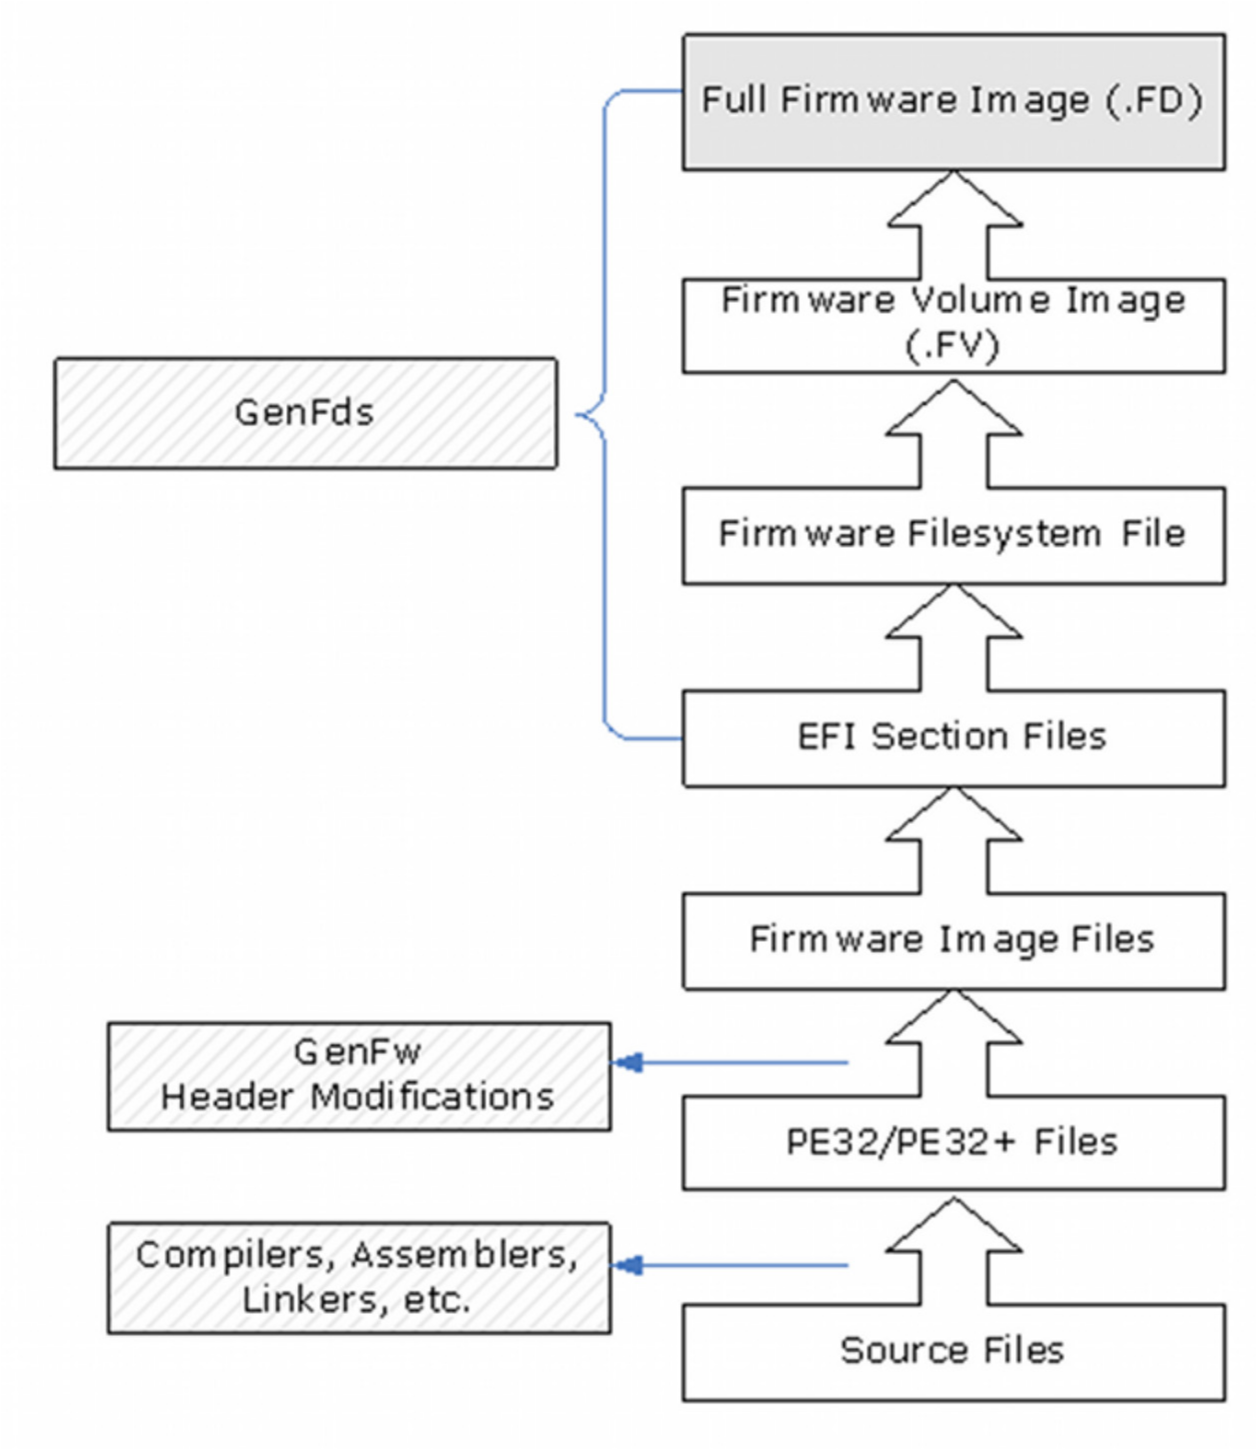
\includegraphics[width=\textwidth]{flash_device}
firmware device
persistent
physical device
contains firmware code and/or data
typically flash
may be divided into smaller pieces to form multiple logical firmware devices
multiple physical firmware devices may be aggregated into one larger logical firmware device

\acf{FV}
logical device
organized into a file system
attributes such as
- size
- formatting
- read/write access

\acf{FFS}
organization of files and free space
no dierectory hierarchy
all files flat in root dir
parsing requires walking for beginning to end

firmware files
types
% PEI_CORE
% PEIM
% DXE_CORE
% DRIVER
% FIRMWARE_VOLUME_IMAGE
% FREEFORM

some file types are sub-divided in file sections

file sections can be either
encapsulation or leaf
leaf sections such as
PE32
% DXE_DEPEX
% PEI_DEPEX
RAW
VERSION
TE

dxe drivers files
contain one PE32 executable section
may contain version section
may contain dxe depex section

freeform files
can contain any combination of sections

PEI phase Service Table
FfsFindNextFile, FfsFindFileByName and FfsGetFileInfo

DXE phase
% EFI_FIRMWARE_VOLUME2_PROTOCOL

depex

\cite{tianocore-edk2-build-spec}

\subsection{\acs{UEFI} Images}

% https://edk2-docs.gitbook.io/edk-ii-build-specification/2_design_discussion/22_uefipi_firmware_images

files containing executable code
subset of PE32+ file format with modified header signature to distinguish from normal PE32 Images
+ stands for addition of 64-bit relocation fix-up extension

relocatable
fixed and dynamic address loading
loaded fully into memory and reloaction fix ups

three different subsystems types: application, boot service driver and runtime service driver
boot and runtime memory

application vs os loader vs driver
memory they reside in
unloaded on return
unloaded on error

memory marked as code and data
jump to entry point

what is the boot manager
boot manager = bds

\subsubsection{\acs{UEFI} Applications}

% https://edk2-docs.gitbook.io/edk-ii-uefi-driver-writer-s-guide/3_foundation/readme.7/371_applications

example efi shell
loaded by boot manager or other applications
return or calling exit specifically
always unloaded from memory

\subsubsection{UEFI OS Loaders}

% https://edk2-docs.gitbook.io/edk-ii-uefi-driver-writer-s-guide/3_foundation/readme.7/371_applications

example windows boot manager
normally take over control from the firmware
upon load behaves like a normal UEFI application
- only use memory allocated from the firmware
- only use services/protocols to access devices that the firmware exposes
- conform to driver specifications to access hardware
on error can return allocated resources with Exit boot service with error specific information given in ExitData
on success take full control with ExitBootServices boot service
all boot services in the system are terminated, including memory management
UEFI OS loader now responsible

\subsubsection{UEFI Drivers}

% https://edk2-docs.gitbook.io/edk-ii-uefi-driver-writer-s-guide/3_foundation/readme.7/372_drivers

loaded by boot manager, UEFI firmware (DXE foundation), or other applications
example payload
unloaded only when returning error code
presistent on success
boot and runtime drivers
only difference is that runtime are available after ExitBootServices was called
boottime drivers are terminated and memory is released
runttime drivers are fixed up with virtual mappings upon SetVirtualAddressMap call
has to convert its allocated memory

\subsection{Firmware Core}
\subsubsection{Systemtable}
% https://edk2-docs.gitbook.io/edk-ii-uefi-driver-writer-s-guide/3_foundation/33_uefi_system_table
system tables offers boot and runtime services
supplied by drivers implementing arichtectural protocols % how to uefi buch zitat
\subsubsection{Handles}
% https://edk2-docs.gitbook.io/edk-ii-uefi-driver-writer-s-guide/3_foundation/36_protocols_and_handles
% https://edk2-docs.gitbook.io/edk-ii-uefi-driver-writer-s-guide/3_foundation/34_handle_database
\cite[7.3 Protocol Handler Services]{uefi-spec}
\subsubsection{Protocols}
% https://edk2-docs.gitbook.io/edk-ii-uefi-driver-writer-s-guide/3_foundation/35_guids
consists of GUID and protocol interface structure containing functions and instance data used to access a device

provide software abstractions for devices such as consoles, mass storage devices and networks
They can also be used to extend the number of generic services that are available in the platform
\cite[2.4 Protocols]{uefi-spec}
boot services provide function to install, locate, open, close and monitor protocols
\cite[7.3 Protocol Handler Services]{uefi-spec}
% https://edk2-docs.gitbook.io/edk-ii-uefi-driver-writer-s-guide/5_uefi_services/51_services_that_uefi_drivers_commonly_use/513_handle_database_and_protocol_services
identified with guids
\subsubsection{Boottime Services}
\subsubsection{Runtime Services}


\subsection{edk2}
build system

BaseTools package process files compiled by third party tools, as well as text and Unicode files in order to create UEFI or PI compliant binary image files
\cite{tianocore-edk2}